\documentclass{article}
\usepackage{a4}
\usepackage{authblk}
\usepackage{pdfpages}
\usepackage{appendix}
\usepackage{graphicx}
\graphicspath{ {./images/} }
\title{Decentralisation of polling processes in developing nations: VoteBlocks Project Report}
\author{Sumuk Shashidhar - 12A \\ Adithya Mahesh -12A}
\affil{Sri Kumaran Children's Home}



\begin{document}
    \maketitle
    \begin{abstract}
        We put forward an idea and a prototype for an open-source, low-power, polling system built on traditional blockchain technology to decentralise the election process in developing nations in order to protect democracy and prevent voter fraud. Simple resource-efficient hashing mechanisms are used in order to ensure energy-efficiency but at the same time rely on the safety in scale approach to preventing attacks in the electoral process. Limitations of the voter-registration process and partial decentralisation problems are carefully examined and solutions are proposed for the same. \\

        \textit{Keywords}— elections, democracy, blockchain, decentralised, crypto
    \end{abstract}
    \pagebreak
    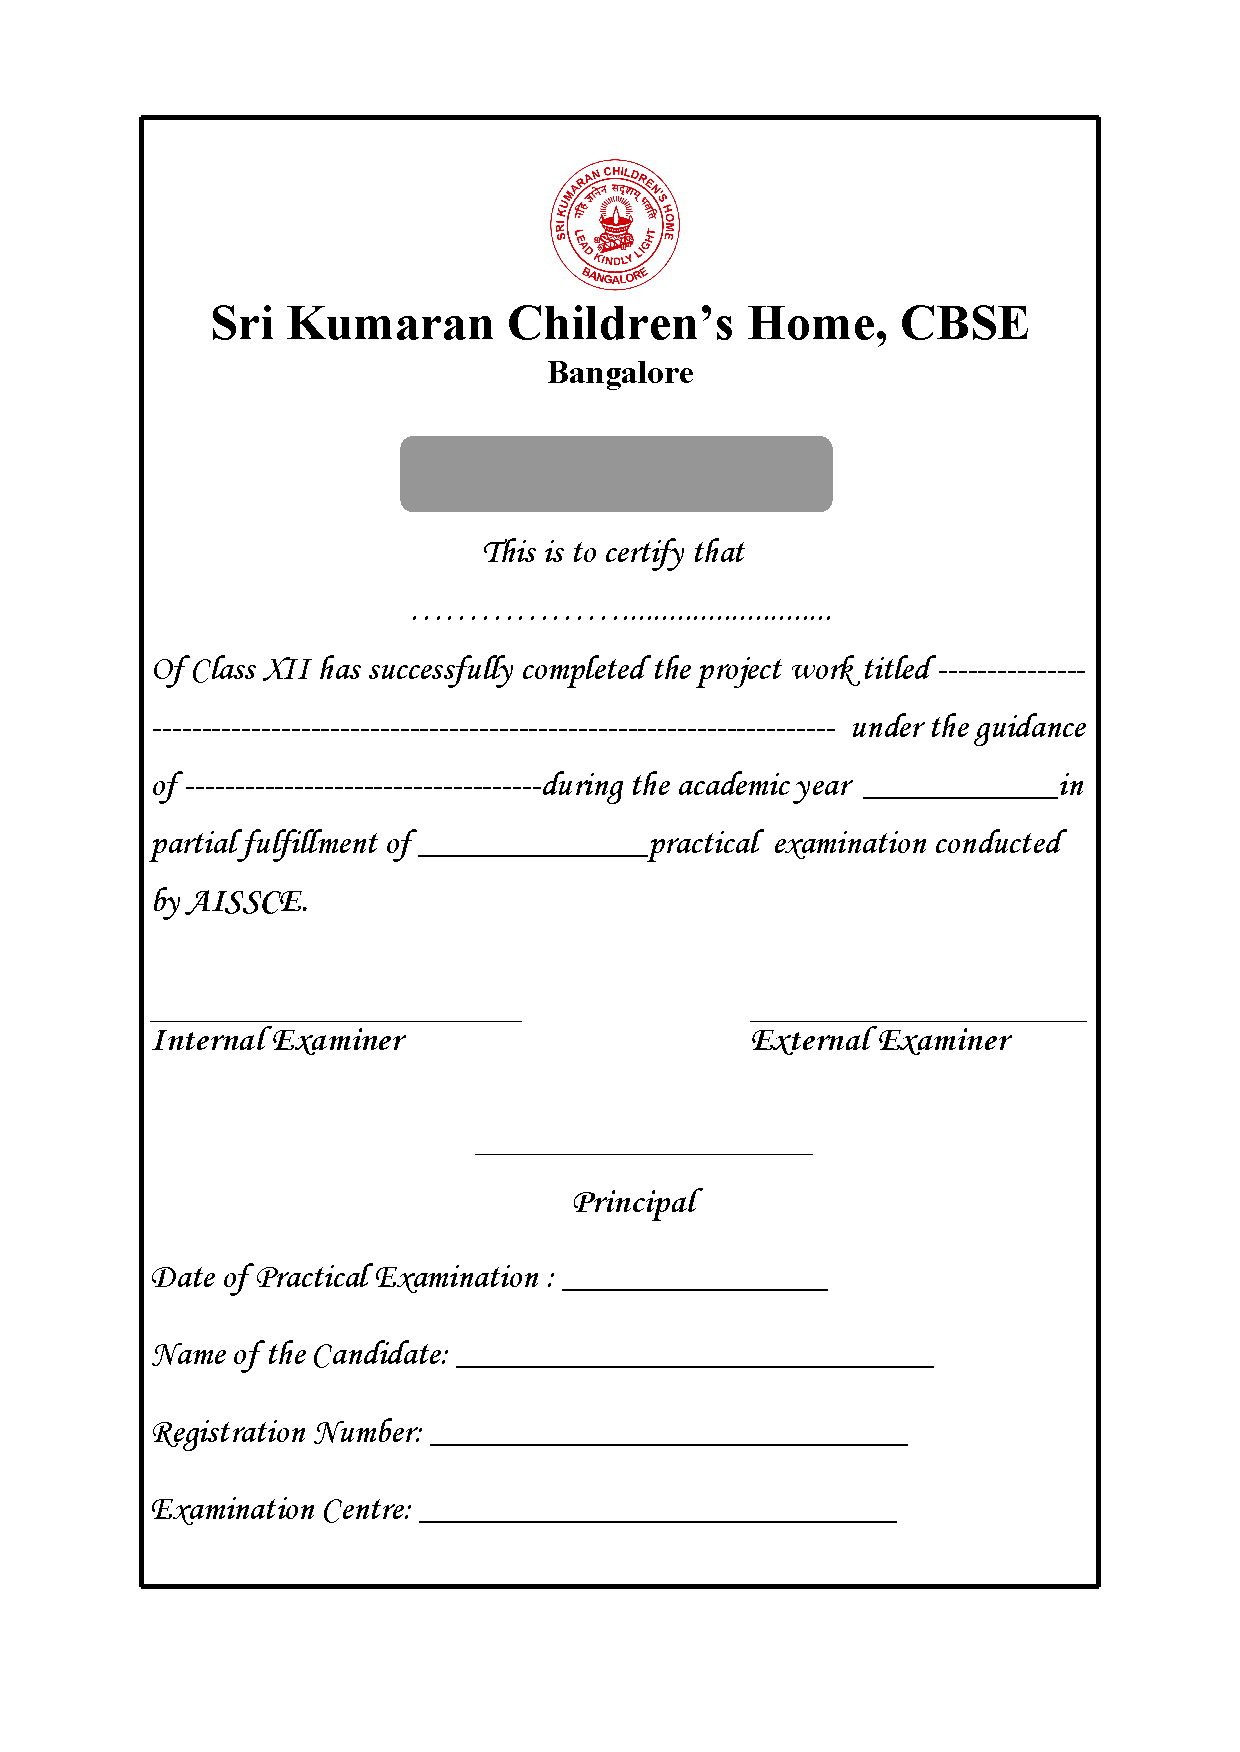
\includepdf[pages=-]{certificate.pdf}
    \section*{\centering Acknowledgements}
    The success of a project depends upon the persistent of an individual and the sustained support received from a few other who are equally responsible for their precious appreciation of such endeavours. My strength is all due to my honourable Principal Deepa Sridhar, who has been an unending source of inspiration and support towards accomplishment of this project. \\

    I would like to express my deepest sense of gratitude towards my computer science teacher Ms. Pavani Kanukollu without whom I could not have successfully completed this project. \\
    
    I would also thank all my friends who helped me create such a project. \\ 
    
    My personal gratitude is extended towards my parents, who have been a constant source of encouragement and support in the sense of this project. Last but not least I want to thank Almighty for enlightening, strengthening and guiding me in the completion of the project.
    \pagebreak
    \tableofcontents
    \pagebreak
    \section{Introduction}
    Democracy in developing nations is often challenged by electoral opacity. A lack of technological advancement/accessibility is a crutch and contributes to widespread voter fraud and voter suppression [1]. To combat this, we propose a decentralised plug-and-play polling system that allows the general public to take part in both aspects of the electoral process: organisation and voting. This also plays a psychological role as it allows the public to personally invest themselves in the process, thereby increasing voter turnouts and national democratic trust.

    VoteBlocks is the proposed prototype that is built on Python and Flask to ensure compatibility with a wide range of available hardware and minimal dependencies [2]. It consists of two parts that can be hot swapped: a frontend web application and a backend server. These can be run on the same machine or independently, thereby ensuring ease of use and greater control. It follows a traditional blockchain approach to recording of anonymous votes and allows any independent party to participate in the electoral process.    
    
    \subsection{The need}
    VoteBlock is a decentralized, trustless voting system built using the concepts of Blockchain. It digitalizes a very important aspect of a democracy’s needs - the receiving, storage and counting of votes in elections. It also addresses the skepticism of security of the same while doing so, as it doesn’t rely on the trust of one single centralized entity which can have control over everything. 
    
    The storage of votes as “hashes” and the decentralized yet consistent nature in which the votes are stored, together ensure the authenticity of the votes and thereby the election results.
    
    The world is moving towards the use of technology to simplify more and more needs. On the other hand, the concerns of security in this matter are on the rise too. This application embraces the use of technology in the process of democratic elections, meanwhile tackling the security concerns too. Every application of Computer Science and this crucial issue is behind our motivation to develop VoteBlocks
    
    \section{System Requirements}
    \begin{itemize}
        \item Hardware
        \subitem Processor: i5 or better
        \subitem RAM: 8 gigabytes or greater
        \item Software
        \subitem Operating System: Any
        \subitem Python: 3.6 or greater
    \end{itemize}
    \section{Project Flow}
    The voting flow consists of two groups of processes that are dealt with in stages: electoral and counting. We put forward stringent yet enforceable guidelines to ensure fair elections.
    \subsection{Electoral Process}
    \subsubsection{Voter Registration}
    All voters must be registered at three separate centres with the same information. The logistical challenges are recognised, but this is crucial to keeping the process fair and democratic. Each centre must follow strict guidelines in the registration of voters, and ask for three separate pieces of identification and proofs of address. After the preliminary registration process, a synchronisation procedure must be conducted to remove inconsistent data and recapture missing or incorrect data. Care must be taken by registration centres to not store or leak personal information, but rather store hashes to ensure individuality while protecting voter anonymity. This is achieved by hashing user details immediately on capture.
    \subsubsection{Polling Process}
    On election day, voters must report to any of the available designated polling centres (the decentralised nature also removes many restrictions currently in place today that enforce the casting of votes to a singular region). Voters must report with their names, their pre-designated password and unique voter-id. Each voter must cast a vote as early as possible (see tallying process). Once the designed block-size limit is achieved, centres must mine the casted votes to add them to the network. These unconfirmed votes will be broadcast on the blockchain to allow public mining for purposes of trust distribution and decentralisation.
    \subsection{Tallying Process}
    Votes are tallied from a first-in first-out principle. For each voter-hash stored, a process is conducted to ensure that there are no other votes cast with a later time-stamp. If such votes exist, they are discarded immediately. This is in accordance with the blockchain double-spending problem solution [3]. A check is then performed to ensure that the corresponding voter-hash exists in more than two registration centre databases. If these tests pass, the vote is tallied towards the total for a candidate.
    The raw data of the blockchain with the specific voter-hashes is then broadcasted to the public to ensure transparency.
    \section{Blockchain Structure}
    The system is broken down into two major components. The block, and the chain. Each chain is made up a number of blocks, all interlinked with each other. Each block is populated with the transactions, i.e., votes in our model. [4]

    When votes are cast, they are added to a list of unconfirmed transactions. When the block is to be mined, it will be put through a SHA-256 function numerous times in order to match a certain hash pattern. Once the right hash is formed using the nonce, it is added to the block.

    When combined, these entities form blockchains, which are hosted and co-ordinated by a number of Python Flask servers, to ensure redundancy. This ensures that the election process can continue with the support of a simple plug-and-play system, where nodes and servers can be swapped out while in operation to fix issues or improve performance. This is beneficial as it provides maximum redundancy while allowing industry-standard operational performance.
    \subsection{Structure of a block}
    Each block consists of the following elements essential to recording votes and identifying individuality of each voter. SHA- 256 hashing is used, where the data of the block is first input into a string, and then computed after being Unicode encoded.
    \begin{itemize}
        \item Index - To enumerate each block
        \item Transactions - The given transactions in each block (votes)
        \item Timestamp - The timestamp of each block's creation
        \item Previous Hash - The hash of the previous block to facilitate the blockchain
        \item Nonce - The number only used once. Used to supplement the rest of the data to generate a desired hash pattern
    \end{itemize}
    \subsection{Structure of the chain}
    We discuss the structure of the chain as a combined product of its properties and functions as listed.
    \subsubsection{Difficulty property}
    The difficulty is a simple integer that determines how hard it is to mine a block. The higher this integer is set, the more difficult it is to mine. This is accomplished by using the number of leading zeros to the hash. A difficulty of 2 will ensure that there are two leading zeros for each accepted hash.
    \subsubsection{Genesis block property}
    The genesis block is the first mined block of that blockchain. Here, we mine it with a list of empty transactions and null (0) data, and we add it to the chain.
    \subsubsection{Last block property}
    A built-in function of the blockchain to retrieve the last added block. Useful in many use-cases to check timestamps and retrieve previous hashes.
    \subsubsection{Add block methodology}
    A simple function to add a block to the blockchain which requires only the block object and the proof of work. The block is verified by checking the proof of work to ensure its validity, and ensuring that the previous block hash of the blockchain, and the previous hash property of the submitted block match.
    \subsubsection{Proof of work function}
    A simple function that tries different nonce values to satisfy the hash pattern requirements set by our difficulty criteria.
    \subsubsection{Add new transaction function}
    Appends a transaction to the unconfirmed transaction chain.
    \subsubsection{Proof verification function}
    The proof is verified by using the hash supplied and the SHA-256 hash computed on the spot.
    \subsubsection{Chain validity check function}
    We use the valid proof check on each and every block in the chain to check if the chain as a whole is valid. It is this process that gives the strength to the blockchain, because it is relatively easy to verify the validity of the chain, compared to creating a fake valid chain from scratch.
    \subsubsection{Mining function}
    A new block is created with the given unconfirmed transactions and the proof of work is computed. The add block method is then used to add the new block to the blockchain, and the unconfirmed transactions / votes are removed.
    \subsection{Structure of the API}
    \subsubsection{New transaction reporting}
    A post request route that allows you to send a candidate choice and a voter-hash, validates the
    requirement, and adds the cast vote into the list of unconfirmed transactions.
    \subsubsection{Chain retrieval}
    A get request route that returns the entire blockchain.
    \subsubsection{Mining}
    A get request route that mines the block, negotiates consensus and announces blocks to the entire network.
    \subsubsection{Registration of new nodes}
    A post request route to register new nodes to the network and add it to a peer list. This internally calls other functions to create chain from data dumps and register with other nodes.
    \subsubsection{Addition of new blocks}
    A post request route to add blocks mined by other entities to the chain. The data is first verified and then added.
    \subsubsection{Pending transaction retrieval}
    A get request route to retrieve all unmined votes.

    \section{Conclusions and further research scope}
    The zero-knowledge structure of the blockchain and the efficacy of the Nakamoto consensus algorithm will ensure anonymous and decentralized elections. However, it is crucial that all stakeholders recognize that the concept of such a fair and decentralized election is subject to a fair registration process by a recognized central agency earlier in the electoral life-cycle. Though there exist various methodologies to decentralize the registration process to ensure end-to-end distribution of control, it is the view of the author that these ideas will not be implementable in countries with massive populations and low technological advancement and accessibility. There is scope for further research regarding implementing an end-to-end decentralized electoral process in developing nations.

    \begin{thebibliography}{9}
        \bibitem{voterfraud} 
        Fund, John H. Stealing elections: How voter fraud threatens our democracy. Encounter Books, 2008.
        
        \bibitem{repo} 
        Shashidhar, S. VoteBlocks. GitHub. https://github.com/sumukshashidhar/voting-blockchain-application, 2021.
        
        \bibitem{doublespend} 
        Hoepman, Jaap-Henk. "Distributed double spending prevention." International Workshop on Security Protocols. Springer, Berlin, Heidelberg, 2007.
        \bibitem{3b1bvideo}
        3Blue1Brown. “But How Does Bitcoin Actually Work?” YouTube, 7 July 2017, www.youtube.com/watch?v=bBC-nXj3Ng4.
    \end{thebibliography}
    \appendix
    \appendixpage
    \addappheadtotoc
    \section*{Appendix 1 - Code written}
    \section*{Appendix 2 - Screenshots}

    \begin{figure}[h]
        \centering
        \includegraphics[width=0.25\textwidth]{mesh}
        \caption{a nice plot}
        \label{fig:mesh1}
    \end{figure}
    

\end{document}